\documentclass[10pt, aspectratio=169]{beamer}

\usetheme[progressbar=frametitle, sectionpage=progressbar, subsectionpage=progressbar, numbering=fraction, block=fill]{metropolis}

\definecolor{mLightBrown}{HTML}{4D4D4D}
\definecolor{mMediumBrown}{HTML}{2C2C2A}
\definecolor{mDarkBrown}{HTML}{1A1A19}
\definecolor{mDarkTeal}{HTML}{0F6E56}
\definecolor{mDarkRed}{HTML}{B03A2E}
\setbeamercolor{normal text}{fg=mDarkBrown}
\setbeamercolor{alerted text}{fg=mDarkTeal}
\setbeamercolor{frametitle}{bg=mDarkBrown}
\setbeamercolor{progress bar}{fg=mDarkTeal, bg=mDarkTeal!20}
\definecolor{mPaleBg}{HTML}{F4F3EE}
\setbeamercolor{block title}{bg=mDarkBrown!10, fg=mDarkBrown}
\setbeamercolor{block body}{bg=mPaleBg, fg=mDarkBrown}
\newcommand{\hl}[1]{\textcolor{mDarkTeal}{#1}}

\usepackage{amsmath, amssymb, amsthm, mathtools}
\usepackage{cancel}\usepackage{bm}\usepackage{booktabs}\usepackage{array}
\usepackage{xcolor}\usepackage{colortbl}\usepackage{multirow}\usepackage{tikz}
\usetikzlibrary{positioning,arrows.meta,calc,fit,shapes.geometric,decorations.pathmorphing}

\newcommand{\paper}[1]{\textcolor{mLightBrown}{\small\textit{(#1)}}}

\newcommand{\qcur}{0}
\newcommand{\qnode}[4]{%
\ifnum#4=\qcur
 \node[draw=mDarkTeal, fill=mDarkTeal!12, thick, rounded corners=1pt, minimum width=3.0cm, minimum height=0.52cm, font=\tiny\bfseries, text=mDarkBrown] (#2) at (#1,0) {#3};%
\else
 \node[draw=mLightBrown!45, rounded corners=1pt, minimum width=3.0cm, minimum height=0.52cm, font=\tiny, text=mLightBrown] (#2) at (#1,0) {#3};%
\fi}
\newcommand{\qstrip}[1]{\renewcommand{\qcur}{#1}%
\begin{center}
\begin{tikzpicture}
\qnode{0}{q1}{Q1 Why a belief?}{1}
\qnode{3.7}{q2}{Q2 Update?}{2}
\qnode{7.4}{q3}{Q3 Pick one?}{3}
\qnode{11.1}{q4}{Q4 Predict?}{4}
\draw[-{Stealth}, mLightBrown!60] (q1.east) -- (q2.west);
\draw[-{Stealth}, mLightBrown!60] (q2.east) -- (q3.west);
\draw[-{Stealth}, mLightBrown!60] (q3.east) -- (q4.west);
\end{tikzpicture}\end{center}}

\title{Fundamentals on Bayesian Statistics}
\subtitle{Don't pick a number --- carry a belief}
\author{Jinkyoo Park}
\institute{KAIST}
\date{\textit{Lecture 2 --- Uncertainty about the model, made into a distribution}}

\begin{document}

\maketitle

%==========================================================
\section{The handoff --- the objective was uncertain}
%==========================================================

\begin{frame}{Where we are --- the model stops being exact}
\vspace{2pt}
\begin{center}\footnotesize\renewcommand{\arraystretch}{1.5}
\begin{tabular}{r|c|c}
 & \textbf{Model-based (certain)} & \textbf{Data-driven (uncertain)} \\
\hline
\textbf{Static, single}  & optimization \scriptsize(Lec.\ 1) & \cellcolor{mDarkTeal!20}\textbf{Bayesian statistics} \scriptsize(\alert{Lec.\ 2})\\
\end{tabular}
\end{center}
\smallskip

Lecture 1 minimized a \emph{known} $f$. But in practice $f$ comes from a \alert{model fit to noisy data} --- its parameters are uncertain. A single ``best'' decision then rests on a single, possibly wrong, parameter estimate.
\smallskip

\pause
So this lecture steps back from \emph{deciding} to \emph{modeling under uncertainty}: how to represent, and update, what we believe about a model's parameters given data. It is the first encounter with the course's central axis --- \alert{from a world handed to us, to a world inferred from data}.
\end{frame}

\begin{frame}{The thesis --- a belief, not a guess}
The fixed point of this lecture, in one line:
\begin{center}\large
\alert{When you don't know a parameter, don't pick one value --- carry a distribution over all of them.}
\end{center}
\medskip

\pause
Two worldviews on an unknown parameter $\theta$:
\begin{center}\footnotesize\renewcommand{\arraystretch}{1.4}
\begin{tabular}{l|l}
\textbf{Frequentist} & \textbf{Bayesian} \\
\hline
$\theta$ is fixed but unknown & $\theta$ is a random variable \\
estimate by maximizing likelihood & estimate a full posterior distribution \\
one point estimate $\hat\theta$ & a balance of prior belief and evidence \\
\end{tabular}
\end{center}
\medskip

\pause
The Bayesian move --- treating the unknown itself as a distribution that data sharpens --- is the engine behind Gaussian processes (Ch 4), surrogate uncertainty (Ch 5), and belief-state decision-making (Ch 3 onward). Learn it once, reuse it all term.
\end{frame}

\begin{frame}{The roadmap --- four questions}
\qstrip{0}
\medskip
\begin{itemize}\setlength\itemsep{3pt}
\item \textbf{Q1 --- Why represent belief as a distribution?} Bayes' rule and the prior--posterior picture.
\item \textbf{Q2 --- How does data update belief?} The posterior as a \alert{balance} of prior and evidence; conjugacy.
\item \textbf{Q3 --- What if I must commit to one value?} MLE vs.\ MAP --- and why \alert{regularization is a prior}.
\item \textbf{Q4 --- How do I predict with my uncertainty intact?} The \alert{posterior predictive} distribution.
\end{itemize}
\end{frame}

%==========================================================
\section{Act 1 --- belief as a distribution}
%==========================================================

\begin{frame}{Bayes' rule --- the whole of inference on one line}
\qstrip{1}
\medskip
\[
\underbrace{p(\theta \mid \text{data})}_{\text{\hl{posterior}}} = \frac{\overbrace{p(\text{data}\mid\theta)}^{\text{likelihood}}\;\overbrace{p(\theta)}^{\text{prior}}}{\underbrace{p(\text{data})}_{\text{evidence}}} \;\propto\; p(\text{data}\mid\theta)\,p(\theta).
\]
\medskip
\begin{itemize}\setlength\itemsep{1pt}
\item \textbf{prior} $p(\theta)$ --- what we believe before seeing data;
\item \textbf{likelihood} $p(\text{data}\mid\theta)$ --- how probable the data is under each $\theta$;
\item \textbf{posterior} $p(\theta\mid\text{data})$ --- updated belief;
\item \textbf{evidence} $p(\text{data}) = \int p(\text{data}\mid\theta)p(\theta)\,d\theta$ --- a normalizing constant.
\end{itemize}
\medskip

\pause
\begin{center}\large
Belief in $=$ prior; belief out $=$ posterior; data does the turning.
\end{center}
This is not a formula to memorize but a \alert{procedure}: choose a model, place a prior, write a likelihood, turn the crank.
\end{frame}

\begin{frame}{The picture --- belief sharpening with evidence}
A flat prior over a coin's bias; each toss reshapes it. With more data the posterior concentrates --- epistemic uncertainty shrinking before our eyes.
\medskip
\begin{center}
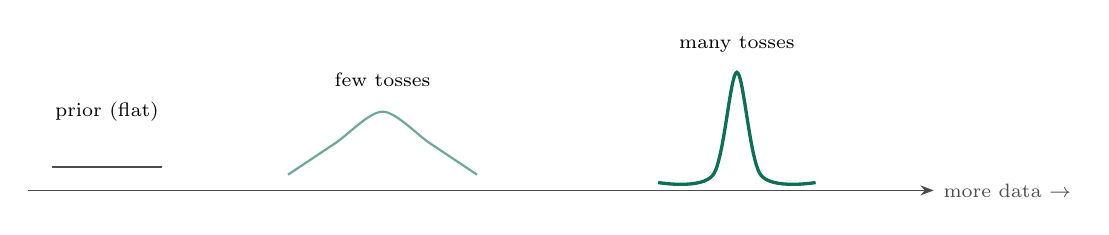
\begin{tikzpicture}[font=\scriptsize]
\draw[-{Stealth}, mLightBrown] (0,0) -- (11.5,0) node[right]{more data $\rightarrow$};
% prior: flat
\draw[mLightBrown, thick] (0.3,0.3) -- (1.7,0.3);
\node at (1.0,1.0) {prior (flat)};
% after few
\draw[mDarkTeal!60, thick] plot[smooth] coordinates {(3.3,0.2)(3.9,0.6)(4.5,1.0)(5.1,0.6)(5.7,0.2)};
\node at (4.5,1.4) {few tosses};
% after many: sharp
\draw[mDarkTeal, very thick] plot[smooth] coordinates {(8.0,0.1)(8.7,0.2)(9.0,1.5)(9.3,0.2)(10.0,0.1)};
\node at (9.0,1.85) {many tosses};
\end{tikzpicture}
\end{center}
\medskip

\pause
Note what a distribution buys that a point estimate cannot: it reports not just \emph{a} value but \alert{how sure we are}. Early on, the posterior is wide --- and an honest decision-maker acts cautiously. That ``width'' becomes the explore/exploit signal of Bayesian optimization (Ch 4).
\end{frame}

%==========================================================
\section{Act 2 --- how data updates belief}
%==========================================================

\begin{frame}{The posterior is a balance --- prior vs.\ evidence}
\qstrip{2}
\medskip
With a conjugate prior, the update is closed-form and \emph{interpretable}. Example: Poisson likelihood, Gamma prior. The posterior mean is
\[
\mathbb{E}[\lambda\mid y] = \frac{\alpha + \sum_i y_i}{\beta + n}
= \underbrace{\frac{\beta}{\beta+n}}_{\text{weight on prior}}\,\mathbb{E}[\lambda]\;+\;\underbrace{\frac{n}{\beta+n}}_{\text{weight on data}}\,\hat\theta_{\mathrm{ML}}.
\]
\medskip

\pause
\begin{center}\large
The posterior mean is a \alert{weighted average} of the prior mean and the data's estimate.
\end{center}
\medskip
\begin{itemize}\setlength\itemsep{1pt}
\item small $n$ (little data): the \emph{prior} dominates --- belief barely moves;
\item large $n$: the \emph{data} dominates --- the prior washes out, $\mathbb{E}[\lambda\mid y]\to\hat\theta_{\mathrm{ML}}$;
\item $\beta$ tunes the \alert{strength} of the prior --- how many ``pseudo-observations'' it is worth.
\end{itemize}
\medskip
\pause
This is the quantitative heart of Bayesian inference: data overrules belief, gradually, in proportion to how much of it there is.
\end{frame}

%==========================================================
\section{Act 3 --- collapsing to a point: MLE, MAP, regularization}
%==========================================================

\begin{frame}{When you must commit --- MLE vs.\ MAP}
\qstrip{3}
\medskip
Sometimes a single number is required. Two principled ways to extract one:
\medskip
\begin{center}\footnotesize\renewcommand{\arraystretch}{1.4}
\begin{tabular}{l|l}
\textbf{Maximum Likelihood (MLE)} & \textbf{Maximum a Posteriori (MAP)} \\
\hline
$\hat\theta = \arg\max_\theta\, p(\text{data}\mid\theta)$ & $\hat\theta = \arg\max_\theta\, p(\theta\mid\text{data})$ \\
ignores the prior & $\propto\;\arg\max_\theta\, p(\text{data}\mid\theta)\,p(\theta)$ \\
the frequentist's point estimate & the posterior's peak \\
\end{tabular}
\end{center}
\medskip

\pause
MAP is MLE \emph{plus a prior term}. With abundant data the two coincide (the likelihood swamps the prior). With scarce data, the prior --- the MAP --- is what keeps the estimate sane.
\medskip
\pause
\begin{center}\large
And that prior term has a familiar face.
\end{center}
\end{frame}

\begin{frame}{The unification --- regularization \emph{is} a prior}
Fit linear regression four ways and they line up exactly.
\medskip
\begin{center}\footnotesize\renewcommand{\arraystretch}{1.45}
\begin{tabular}{l|l|l}
\textbf{Estimator} & \textbf{Optimization view} & \textbf{Bayesian view (MAP with prior)} \\
\hline
ordinary least squares & $\min_w \|y - Xw\|_2^2$ & MLE, Gaussian noise, no prior \\
\textbf{Ridge} & $\min_w \|y - Xw\|_2^2 + \lambda \|w\|_2^2$ & MAP, \alert{Gaussian} prior on $w$ \\
\textbf{Lasso} & $\min_w \|y - Xw\|_2^2 + \lambda \|w\|_1$ & MAP, \alert{Laplace} prior on $w$ \\
\end{tabular}
\end{center}
\medskip

\pause
\begin{block}{The punchline}
\centering
A regularizer is not an ad-hoc penalty --- it is the \alert{log of a prior}. \\
Ridge's $\ell_2$ penalty $=$ a Gaussian prior; Lasso's $\ell_1$ penalty $=$ a Laplace prior (which prefers sparsity).
\end{block}
\medskip

\pause
This is the lecture's deepest bridge: \alert{the optimization world and the Bayesian world are the same world}, viewed through different lenses. ``Add a penalty to avoid overfitting'' and ``encode a prior belief about the weights'' are one act.
\end{frame}

%==========================================================
\section{Act 4 --- predicting with uncertainty intact}
%==========================================================

\begin{frame}{Full Bayes --- integrate, don't plug in}
\qstrip{4}
\medskip
MLE/MAP collapse the posterior to a point, then predict --- discarding all uncertainty. The fully Bayesian prediction \alert{averages over the entire posterior}:
\[
p(y^* \mid x^*, \text{data}) = \int p(y^*\mid x^*,\theta)\; \underbrace{p(\theta\mid\text{data})}_{\text{posterior}}\; d\theta.
\]
\medskip

\pause
\begin{center}\large
Don't predict with the \emph{best} $\theta$ --- predict with \emph{all} $\theta$, weighted by belief.
\end{center}
\medskip
\begin{itemize}\setlength\itemsep{1pt}
\item this \alert{propagates uncertainty} into the prediction: the predictive distribution is wider when the posterior is wider;
\item it guards against overconfidence from a single fitted parameter;
\item the price is the integral --- solvable in closed form for conjugate models, otherwise approximated by \alert{sampling} (MCMC) or variational methods.
\end{itemize}
\medskip
\pause
{\footnotesize\textcolor{mLightBrown}{When the ``parameter'' is an entire function, this predictive integral becomes Gaussian-process regression --- the core of Lecture 4.}}
\end{frame}

%==========================================================
\section{Closing}
%==========================================================

\begin{frame}{Where we are --- belief established, complexity ahead}
\vspace{2pt}
\begin{center}\footnotesize\renewcommand{\arraystretch}{1.5}
\begin{tabular}{r|c|c}
 & \textbf{Model-based} & \textbf{Data-driven} \\
\hline
\textbf{Static, single}  & optimization \;{\scriptsize Lec.\ 1 \checkmark} & \cellcolor{mDarkTeal!15}\textbf{Bayesian statistics} \;{\scriptsize Lec.\ 2 \checkmark} $\to$ Lec.\ 3--4\\
\end{tabular}
\end{center}
\medskip

\pause
We can now hold and update a belief over a parameter, collapse it when forced (MLE/MAP), and predict with it intact (full Bayes). But we modeled belief over \alert{one parameter (vector)}.
\medskip

\pause
Real systems have \emph{many} interacting random variables --- failures that cause failures, symptoms that imply causes. A joint distribution over them is exponentially large. How do we represent, and reason within, belief over a whole system?
\begin{center}\large
That is Lecture 3: \alert{a belief about many things is a graph.}
\end{center}
\end{frame}

\begin{frame}{Closing --- the one sentence}
\vfill
\begin{center}\large
Frequentists estimate a number; Bayesians carry a distribution ---\\[8pt]
a prior turned by data into a posterior,\\[4pt]
collapsed to a point only when forced (and even then, a prior in disguise),\\[4pt]
and integrated over when prediction must stay honest.
\end{center}
\vfill
\pause
\footnotesize
The single idea --- \emph{the unknown is itself a distribution that data sharpens} --- is the seed of everything data-driven this term. Regularization was a prior; a Gaussian process will be a prior over functions; a belief state will be a prior carried through time.
\end{frame}

\begin{frame}[standout]
Questions?
\end{frame}

%==========================================================
\appendix
%==========================================================

\begin{frame}{Backup 1 --- conjugacy, in general}
\footnotesize
A prior is \alert{conjugate} to a likelihood if the posterior belongs to the same family as the prior --- so the update is closed-form (no integral to evaluate).
\medskip
\begin{center}\scriptsize\renewcommand{\arraystretch}{1.35}
\begin{tabular}{l|l|l}
\textbf{Likelihood} & \textbf{Conjugate prior} & \textbf{Posterior} \\
\hline
Bernoulli / Binomial & Beta$(\alpha,\beta)$ & Beta$(\alpha + \#\text{heads},\ \beta + \#\text{tails})$ \\
Poisson & Gamma$(\alpha,\beta)$ & Gamma$(\alpha + \sum y_i,\ \beta + n)$ \\
Gaussian (known var.) & Gaussian & Gaussian \\
\end{tabular}
\end{center}
\medskip
In every case the posterior parameters are the prior's \emph{plus} sufficient statistics of the data --- which is why the posterior mean is always a prior-vs-data weighted average, and why the prior acts like a stock of ``pseudo-observations.'' Conjugacy is the analytic backbone; when it fails, we sample (MCMC) or approximate (variational inference).
\end{frame}

\begin{frame}{Backup 2 --- Lasso as MAP with a Laplace prior}
\footnotesize
Gaussian likelihood $p(y\mid X,w) = \prod_i \mathcal{N}(y_i \mid w^\top x_i, \sigma^2)$, Laplace prior $p(w) = \prod_k \tfrac{\lambda}{2\tau^2}\exp(-\tfrac{\lambda}{\tau^2}|w_k|)$.
\medskip

Posterior $\propto$ likelihood $\times$ prior; take logs:
\[
\log p(w\mid X,y) = -\frac{1}{2\sigma^2}\sum_i (y_i - w^\top x_i)^2 \;-\; \frac{\lambda}{\tau^2}\sum_k |w_k| \;+\; \text{const}.
\]
Maximizing over $w$ (MAP) is therefore
\[
\hat w = \arg\max_w \log p(w\mid X,y) = \arg\min_w \|y - Xw\|_2^2 + \lambda_1 \|w\|_1, \qquad \blacksquare
\]
which is exactly Lasso. The Gaussian prior gives the $\ell_2$ (Ridge) penalty by the identical argument. \textbf{Why $\ell_1$ is sparse:} the Laplace prior places more mass at zero (a sharp peak), so the MAP pushes weak coefficients exactly to $0$ --- automatic feature selection from a belief.
\end{frame}

\begin{frame}{Backup 3 --- linear regression, four ways (one answer)}
\footnotesize
The same fit, derived from four starting points --- a microcosm of the optimization $\leftrightarrow$ Bayes unification:
\begin{enumerate}\setlength\itemsep{2pt}
\item \textbf{Normal equation (optimization):} $\min_w\|y-Xw\|_2^2 \Rightarrow \hat w = (X^\top X)^{-1}X^\top y$.
\item \textbf{MLE (frequentist):} with Gaussian noise, maximizing $\prod_i \mathcal{N}(y_i\mid w^\top x_i,\sigma^2)$ gives the \emph{same} $\hat w$ --- least squares \emph{is} Gaussian-noise MLE.
\item \textbf{MAP (Bayesian point):} add a Gaussian prior on $w$ $\Rightarrow$ Ridge, $\hat w = (X^\top X + \lambda I)^{-1}X^\top y$ --- the prior regularizes the inverse.
\item \textbf{Full Bayes:} keep the whole Gaussian posterior over $w$; predict by integrating it out $\Rightarrow$ a predictive \emph{distribution} with error bars, not a point.
\end{enumerate}
\medskip
\textbf{The lesson.} ``Fit a line'' is a single act seen four ways. As data grows, MLE/MAP/full-Bayes agree on the mean; what full Bayes adds, and the others throw away, is the \emph{uncertainty} --- precisely what Lecture 4 will exploit to decide where to sample next.
\end{frame}

\end{document}
